\documentclass[10pt,twocolumn,letterpaper]{article}

\usepackage{cvpr}
\usepackage{times}
\usepackage{epsfig}
\usepackage{graphicx}
\usepackage{amsmath}
\usepackage{amssymb}
\usepackage{caption}
\usepackage{subcaption}
% Include other packages here, before hyperref.

% If you comment hyperref and then uncomment it, you should delete
% egpaper.aux before re-running latex.  (Or just hit 'q' on the first latex
% run, let it finish, and you should be clear).
\usepackage[breaklinks=true,bookmarks=false]{hyperref}

\cvprfinalcopy % *** Uncomment this line for the final submission

\def\cvprPaperID{****} % *** Enter the CVPR Paper ID here
\def\httilde{\mbox{\tt\raisebox{-.5ex}{\symbol{126}}}}

% Pages are numbered in submission mode, and unnumbered in camera-ready
%\ifcvprfinal\pagestyle{empty}\fi
\pagenumbering{gobble}
\begin{document}

%%%%%%%%% TITLE
\title{Texture Synthesis and Style Transfer}

\author{Aman Kansal\\
170050027\\
\and
Ansh Khurana\\
170050035\\
\and
Kushagra Juneja\\
170050041
}

\maketitle
%\thispagestyle{empty}

% %%%%%%%%% ABSTRACT
% \begin{abstract}
   
% \end{abstract}

%%%%%%%%% BODY TEXT
\section{Introduction}
refer abstract-intro from paper. Here we solve the problem of synthesizing a large image following the given input texture. Also, transferring the texture to another image.  
\begin{figure}[h]
\begin{center}
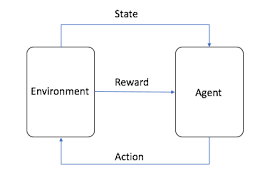
\includegraphics[scale=0.50]{resources/rl_general.png}
\end{center}
\vspace{-0.2em}
\caption{Reinforcement Learning Paradigm}
\label{fig:basic}
\end{figure}
%-------------------------------------------------------------------------
\vspace{-6pt}
\section{Method}

\subsection{Quilting}
Explain algo. Maybe add pseudocode in an algorithm block. Add figure with minimum boundary cut to explain the algo.
\begin{figure}[h]
\begin{center}
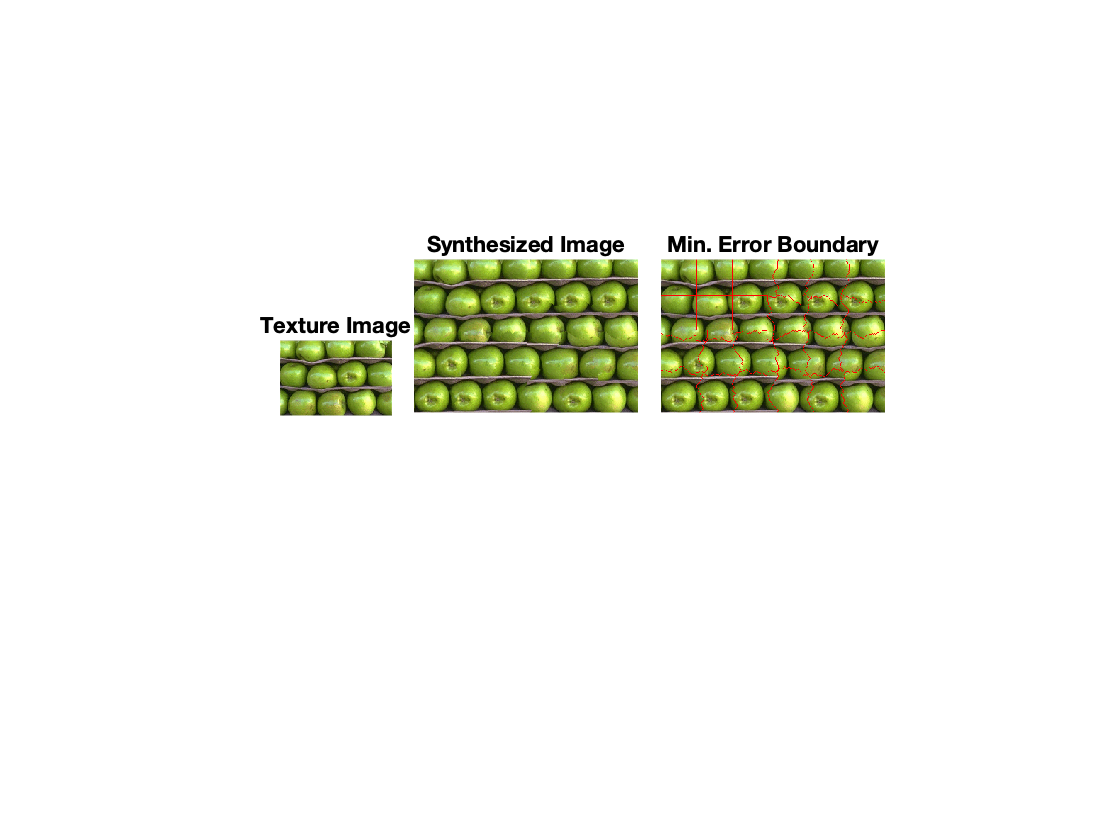
\includegraphics[trim={9cm 15cm 2cm 8cm},clip, scale=0.38]{resources/apple_boundary_example.png}
\end{center}
\vspace{-0.2em}
\caption{Boundary Cuts in Synthesis of Apple image}
\label{fig:bcut_example}
\end{figure}
% \begin{align*}
%     Q_{n}(s, a) = \left(1-\alpha_{n}\right) Q_{n-1}(s, a)+\alpha_{n}\left[r_{n}+\gamma V_{n-1}\left(y_{n}\right)\right]
% \end{align*}
%-------------------------------------------------------------------------
\subsection{Texture Transfer}

In the Approximate Q-Learning approach, the model the agent learns weights for features of states, where many states might share the same features. Function approximation learns the weights of different features during training. Using function approximation for parameterizing the problem of Q-Learning significantly reducing training time. It is important to recognize significant features on which the expected gain for the state will depend. For example, for approximating the Q-function for the Pac-Man game would depend upon features like Distance to closest ghost or dot, number of ghosts nearby, proximity to walls etc. Considering a linear model in the features, the update equations for the weights is given by:
% \vspace{-10pt}
% \begin{align*}

%     Q(s, a) &= \sum_{i=1}^{n} f_{i}(s, a) w_{i}
    
%     \text {difference}=&\left(r+\gamma \max _{a^{\prime}} Q\left(s^{\prime}, a^{\prime}\right)\right)-Q(s, a)
    
%      &w_{i} &\leftarrow w_{i}+\alpha \cdot  \text {difference} \cdot f_{i}(s, a) 
% \end{align*}
%-------------------------------------------------------------------------
\subsection{Neural Network Style Transfer}
% Insert picture of the model
Deep Learning does away with the need to handcraft features for the states. In the Deep Q-Learning based approach, the state is captured by an image of the current situation of the game. %We create an image representing the current state of the game every four frames which are blended together and preprocessed.
Deep Q-Learning is an extension of function approximation for Q-Learning. Deep Q-Learning uses a deep neural network to approximate the Q values for every action, given the current state. Thus, the output layer of the Deep Q-Network has dimensions = $|A|$ (The number of actions). The best action after learning the network can be taken by calculating an argmax over the output layer. 

\begin{figure}[h]
\begin{center}
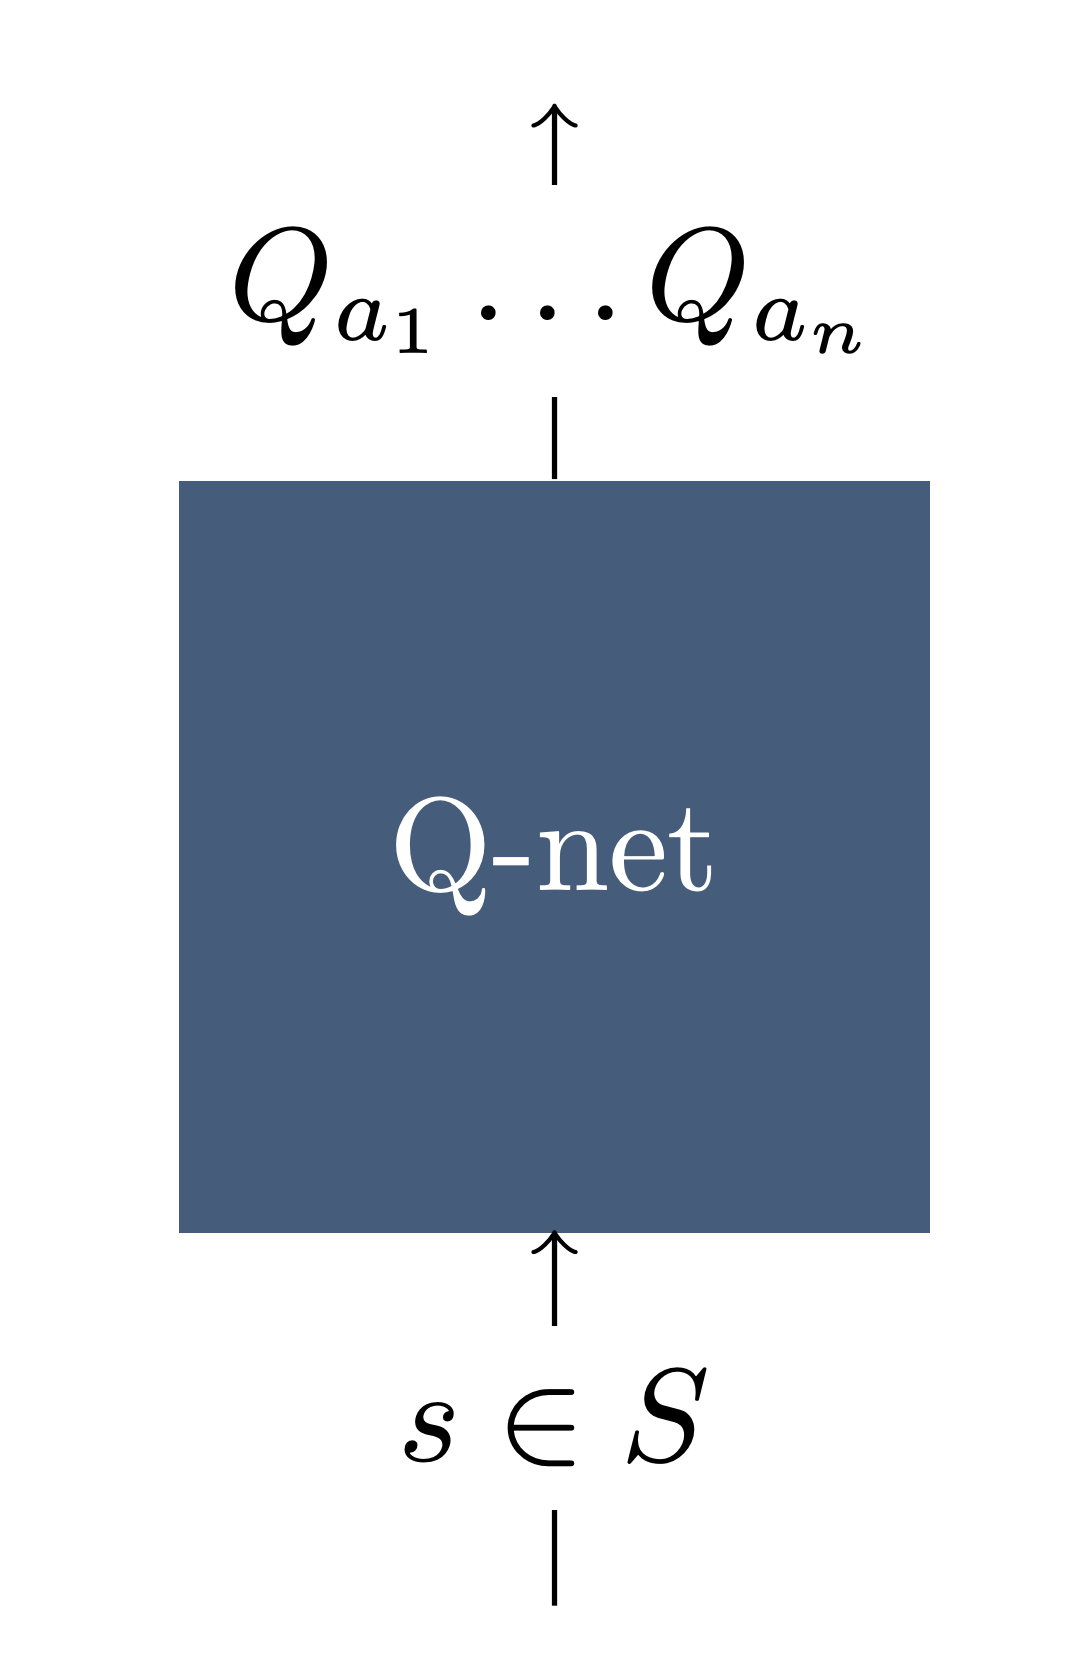
\includegraphics[scale=0.15]{resources/generalQnetwork.png}
\end{center}
\vspace{-0.2em}
\caption{A generic Deep Q-Network}
\label{fig:genericDQN}
\end{figure}
%-------------------------------------------------------------------------


% \begin{table}
% \begin{center}
% \begin{tabular}{|l|c|}
% \hline
% Method & Frobnability \\
% \hline\hline
% Theirs & Frumpy \\
% Yours & Frobbly \\
% Ours & Makes one's heart Frob\\
% \hline
% \end{tabular}
% \end{center}
% \caption{Results.   Ours is better.}
% \end{table}

%-------------------------------------------------------------------------
% \section{Experiments}
% \subsection{Synthesis - Effect of increasing block size}

% An MDP is defined by set of {S, A, T, R} where\\
% S: State Space i.e. set of all possible states ‘s’\\
% A: Action Space i.e. set of all possible states ‘a’\\
% R: Reward for being in a state\\
% T: Transition dynamics/ Probability transition Matrix\\
% In our current formulation of MDP a state is a function of Pac-Man position, ghost position and dots position. Each state is assigned a number between 0 to NumStates-1 so that it uniquely determines the value of all three functions. Action Space ‘A’ is {East, West, North, South}. Reward values are defined such that the maximum positive reward is obtained on eating the dots and negative reward on getting eaten by ghost and idle movements. The only valid transitions end up in a non-blocking grid location with probability with due to only one final state possible for each action.

% \subsection{Joint Training}
% According to the concept of joint training for Pac-Man and ghost we increase the level of Pac-Man by training it on the most intelligent ghost. Similarly, we train the next level using previously trained Pac-Man. So level n+1 of Pac-Man is obtained by training on MDP obtained using ghost policy of level n. Similarly level n of ghost is obtained by training on MDP obtained using Pac-Man policy of level n. We apply value iteration algorithm to obtain Pac-Man policy for MdpPac-Man until it convergers.
%------------------------------------------------------------------------
\section{Experiments}
% Add parameters chosen and values of different things learning rate
\subsection{Synthesis - Effect of block size}

\begin{figure*}[h]
    \centering
    \begin{subfigure}[h]{0.2\textwidth}
        \centering
        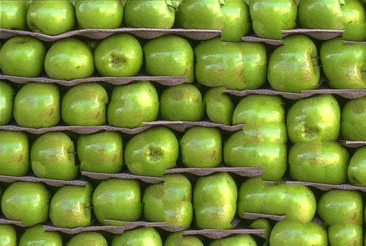
\includegraphics[scale=0.25]{../results/syn/out_apples_B_20.png}
        \caption{B=20}
    \end{subfigure}
    \hfill
    \begin{subfigure}[h]{0.2\textwidth}
       \centering
       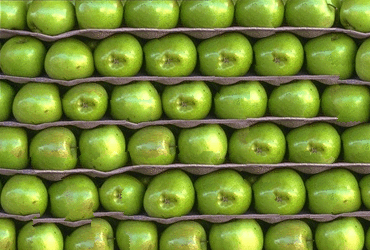
\includegraphics[scale=0.25]{../results/syn/out_apples_B_30.png}
       \caption{B=30}
   \end{subfigure}
   \hfill
   \begin{subfigure}[h]{0.2\textwidth}
       \centering
       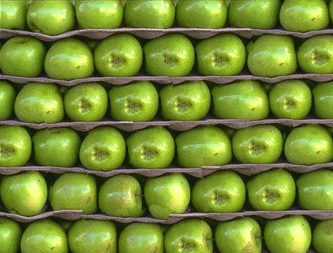
\includegraphics[scale=0.25]{../results/syn/out_apples_B_40.png}
       \caption{B=40}
   \end{subfigure}
   \begin{subfigure}[h]{0.2\textwidth}
       \centering
       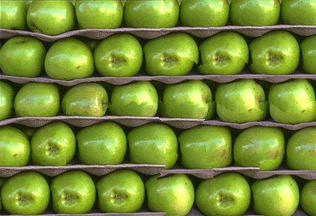
\includegraphics[scale=0.25]{../results/syn/out_apples_B_50.png}
       \caption{B=50}
   \end{subfigure}
   \caption{Effect of block size on Apples}
   \label{fig:ap_bs}
\end{figure*}

\begin{figure*}[h]
    \centering
    \begin{subfigure}[h]{0.2\textwidth}
        \centering
        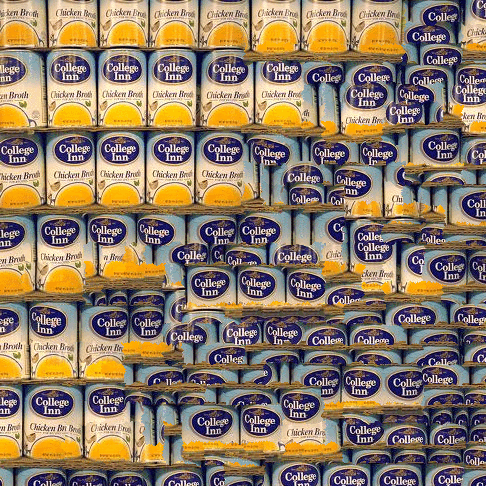
\includegraphics[scale=0.15]{../results/syn/out_cans_B_20.png}
        \caption{B=20}
    \end{subfigure}
    \hfill
    \begin{subfigure}[h]{0.2\textwidth}
       \centering
       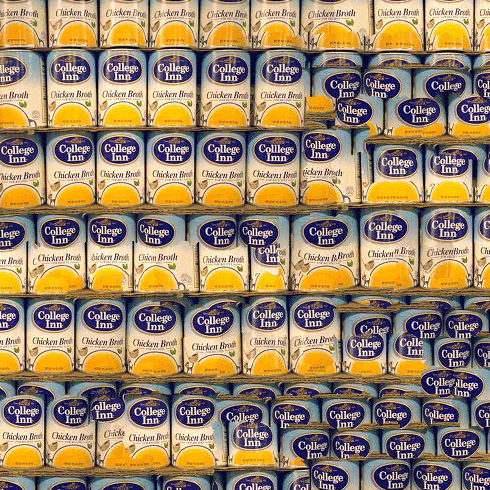
\includegraphics[scale=0.15]{../results/syn/out_cans_B_30.png}
       \caption{B=30}
   \end{subfigure}
   \hfill
   \begin{subfigure}[h]{0.2\textwidth}
       \centering
       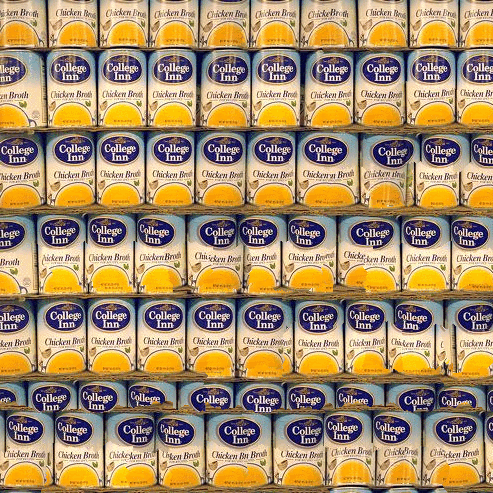
\includegraphics[scale=0.15]{../results/syn/out_cans_B_40.png}
       \caption{B=40}
   \end{subfigure}
   \begin{subfigure}[h]{0.2\textwidth}
       \centering
       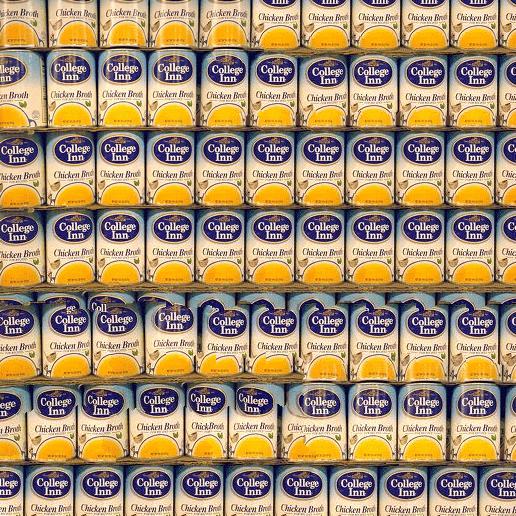
\includegraphics[scale=0.15]{../results/syn/out_cans_B_50.png}
       \caption{B=50}
   \end{subfigure}
   \caption{Effect of block size on Cans}
   \label{fig:cans_bs}
\end{figure*}

\begin{figure*}[h]
    \centering
    \begin{subfigure}[h]{0.2\textwidth}
        \centering
        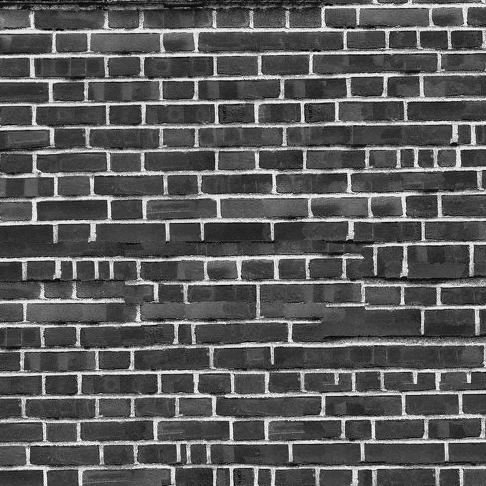
\includegraphics[scale=0.15]{../results/syn/out_brick_bw_B_20.png}
        \caption{B=20}
    \end{subfigure}
    \hfill
    \begin{subfigure}[h]{0.2\textwidth}
       \centering
       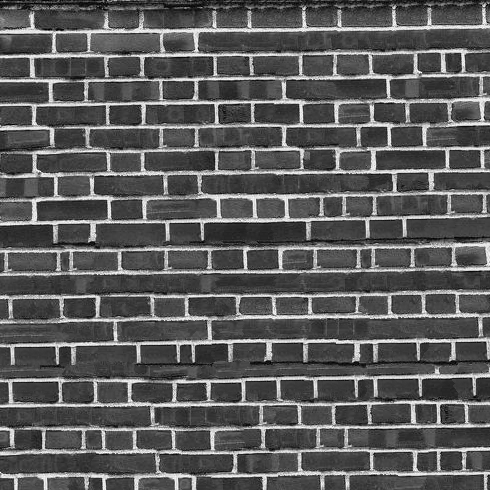
\includegraphics[scale=0.15]{../results/syn/out_brick_bw_B_30.png}
       \caption{B=30}
   \end{subfigure}
   \hfill
   \begin{subfigure}[h]{0.2\textwidth}
       \centering
       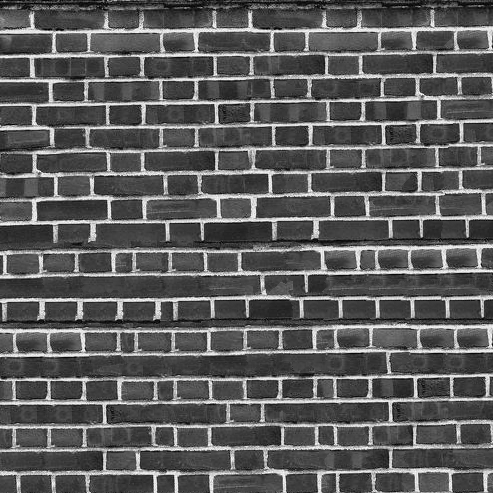
\includegraphics[scale=0.15]{../results/syn/out_brick_bw_B_40.png}
       \caption{B=40}
   \end{subfigure}
   \begin{subfigure}[h]{0.2\textwidth}
       \centering
       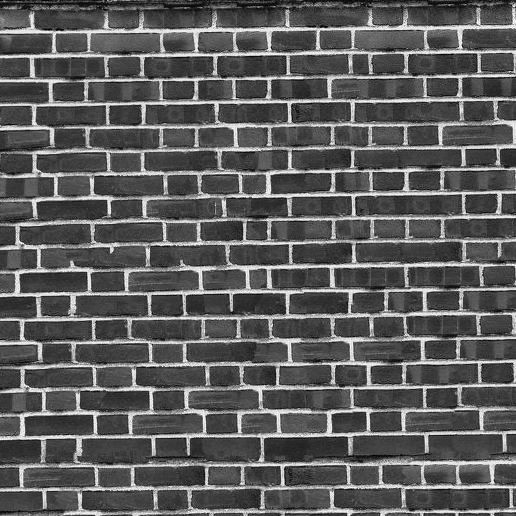
\includegraphics[scale=0.15]{../results/syn/out_brick_bw_B_50.png}
       \caption{B=50}
   \end{subfigure}
   \caption{Effect of block size on Bricks}
   \label{fig:cans_bs}
\end{figure*}

% \begin{table}[!th]
% \begin{center}
% \begin{tabular}{|l|c|}
% \hline
% Situation & Reward \\
% \hline\hline
% Win (finish food) & +500 \\
% Lose (eaten by ghost) & -500 \\
% Eat food & +10\\
% Consume ghost & +200\\
% Idle/no food & -1\\
% \hline
% \end{tabular}
% \end{center}
% \caption{Game parameters for Q-Learning}
% \end{table}
% The features chosen for training the Approximate Q-Learning Network are: bias, number\_of\_ghosts\_1\_step\_away, distance\_to\_closest\_food
% \begin{table}[!th]
% \begin{center}
% \begin{tabular}{|l|c|c|c|c|}
% \hline
% Approach & Grid size & Avg Score & \#Epochs & Time (train)\\
% \hline\hline
% AQL & mediumClassic & 1202.7 & 50 & 5m 45s\\
% AQL & mediumGrid & 526.4 & 50 & 32s \\
% QL & smallGrid & 499.5 & 2000 & 1m 24s\\
% \hline
% \end{tabular}
% \end{center}
% \caption{Some simulations}
% \label{tab:qlres}
% \end{table}


% \begin{figure}[h]
% \begin{center}
% 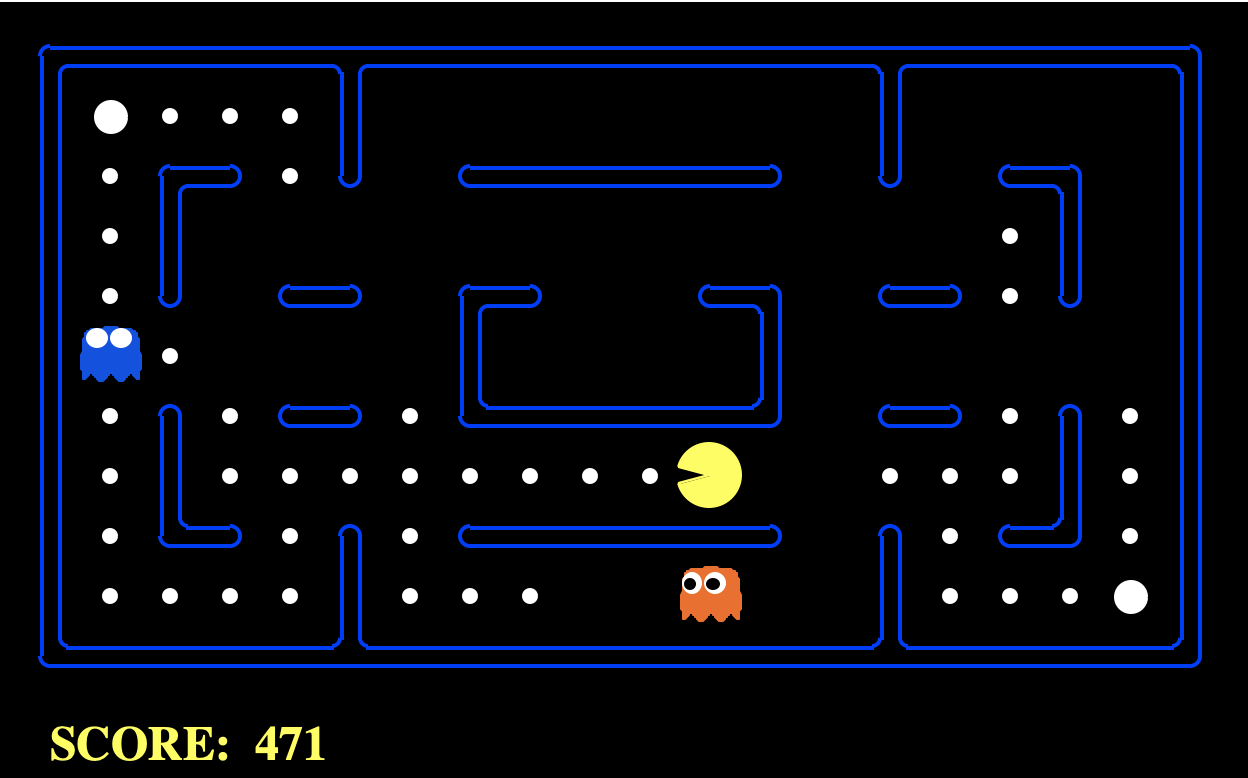
\includegraphics[scale=0.25]{resources/game_preview.png}
% \end{center}
% \vspace{-0.2em}
% \caption{Pac-Man during Training}
% \label{fig:basic}
% \end{figure}

\subsection{Transfer}
We use OpenAI's MsPacman-v0 environment to train a DQN based agent. Here, we use a neural network to approximately calculate the Q values corresponding to a given state which will be given as an input image.\\
The first three layers of the architecture are convolutional layers. The first layer has 32 filters of size 8*8 with stride 4. The second layer has 64 filters of size 4*4 with stride 2. The third layer has 64 filters of size 3*3 with stride 1. The fourth layer is fully connected 512 hidden nodes. The last layer is fully connected too with 9 output nodes corresponding to each of the actions possible.\\
We have used concepts like Replay memory and Epsilon greedy to help our model train better.



\section{Results \& Conclusion}
In this project, we tested a wide range of common reinforcement learning techniques. The Deep Q-Learning based model, the network learns important features from game-state images and thus, approximates Q values by experience. Given enough training time and model complexity, the network can learn and improve upon the game. However, computational cost for the Deep Neural Network is a major concern. As compared to Approximate Q-Learning, Q-Learning takes a much larger number of epochs to gain similar performance. Thus, Q-Learning is not scale-able for large grids.  We find that approximate Q-Learning outperforms the Q-Learning based agent and also trains faster than both the above approaches. Thus, it may be the ideal approach for medium load reinforcement learning tasks like learning how to play Pac-Man on a medium sized grid.\\


\begin{figure*}
     \centering
     \begin{subfigure}[h]{0.33\textwidth}
         \centering
         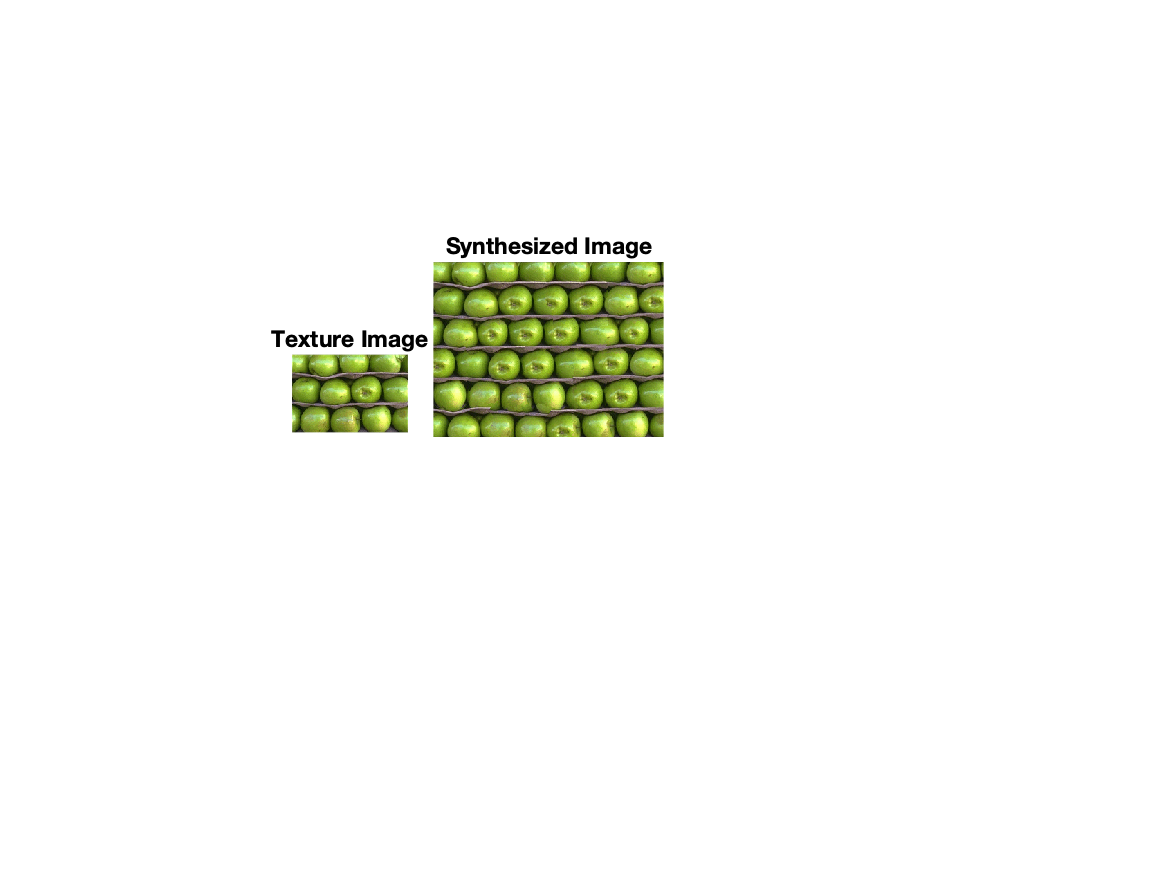
\includegraphics[trim={4.5cm 7cm 8.0cm 3cm}, clip, scale=1.5, width=\textwidth]{../results/syn_final/result_apples_c_B_40.png}
         \caption{Apples}
         \label{fig:apples_res}
     \end{subfigure}
     \hfill
     \begin{subfigure}[h]{0.33\textwidth}
        \centering
        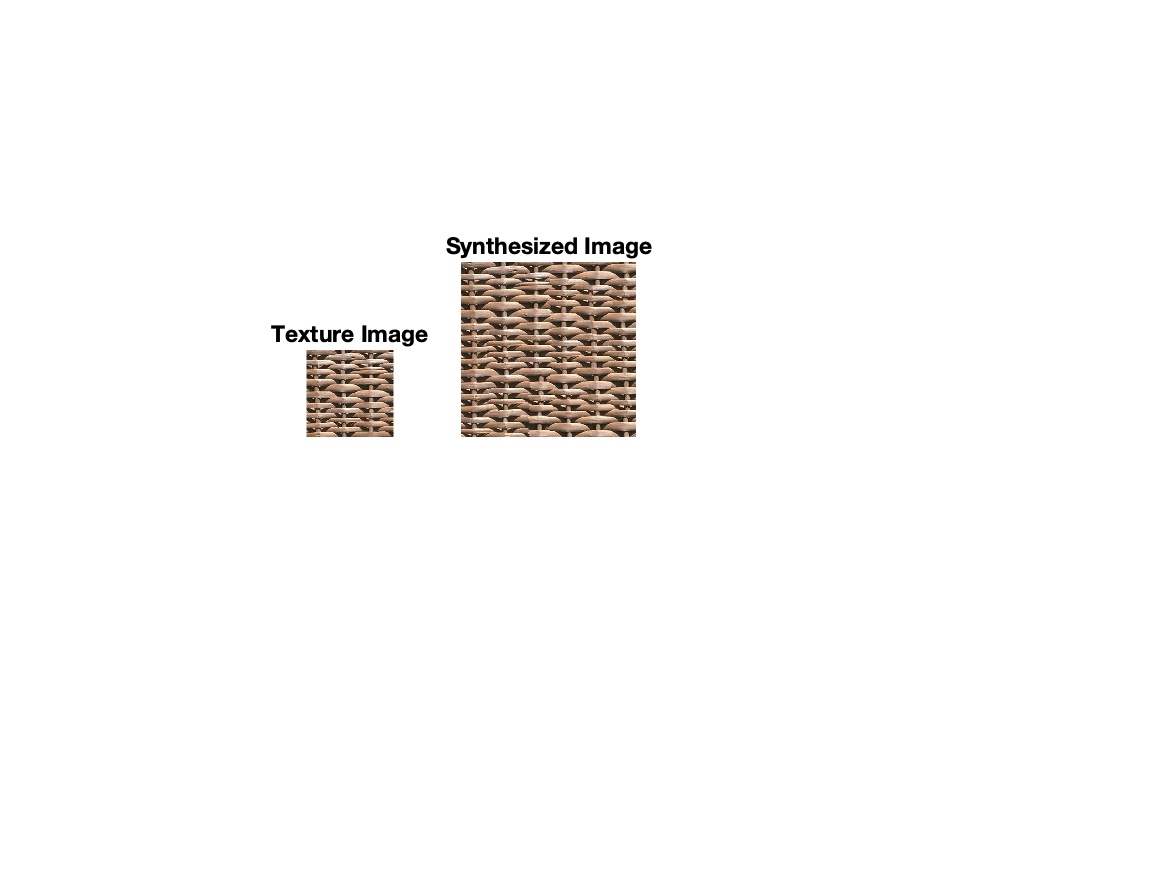
\includegraphics[trim={4.5cm 7cm 8.0cm 3cm}, clip, scale=1.5, width=\textwidth]{../results/syn_final/result_jute_c_B_40.png}
        \caption{Jute}
        \label{fig:jute_res}
    \end{subfigure}
    \hfill
    \begin{subfigure}[h]{0.33\textwidth}
        \centering
        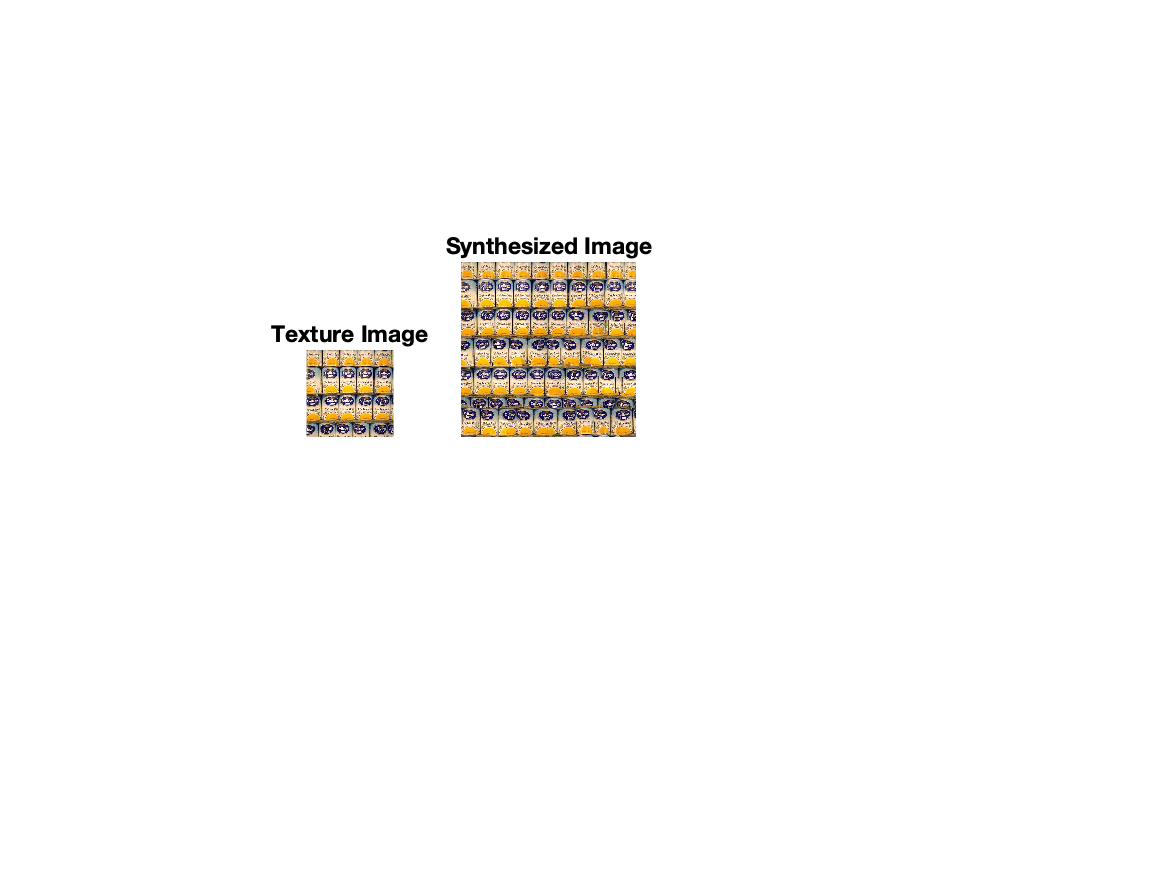
\includegraphics[trim={4.5cm 7cm 8.0cm 3cm}, clip, scale=1.5, width=\textwidth]{../results/syn_final/result_cans_B_40.png}
        \caption{Cans}
        \label{fig:cans_res}
    \end{subfigure}
    \begin{subfigure}[h]{0.33\textwidth}
        \centering
        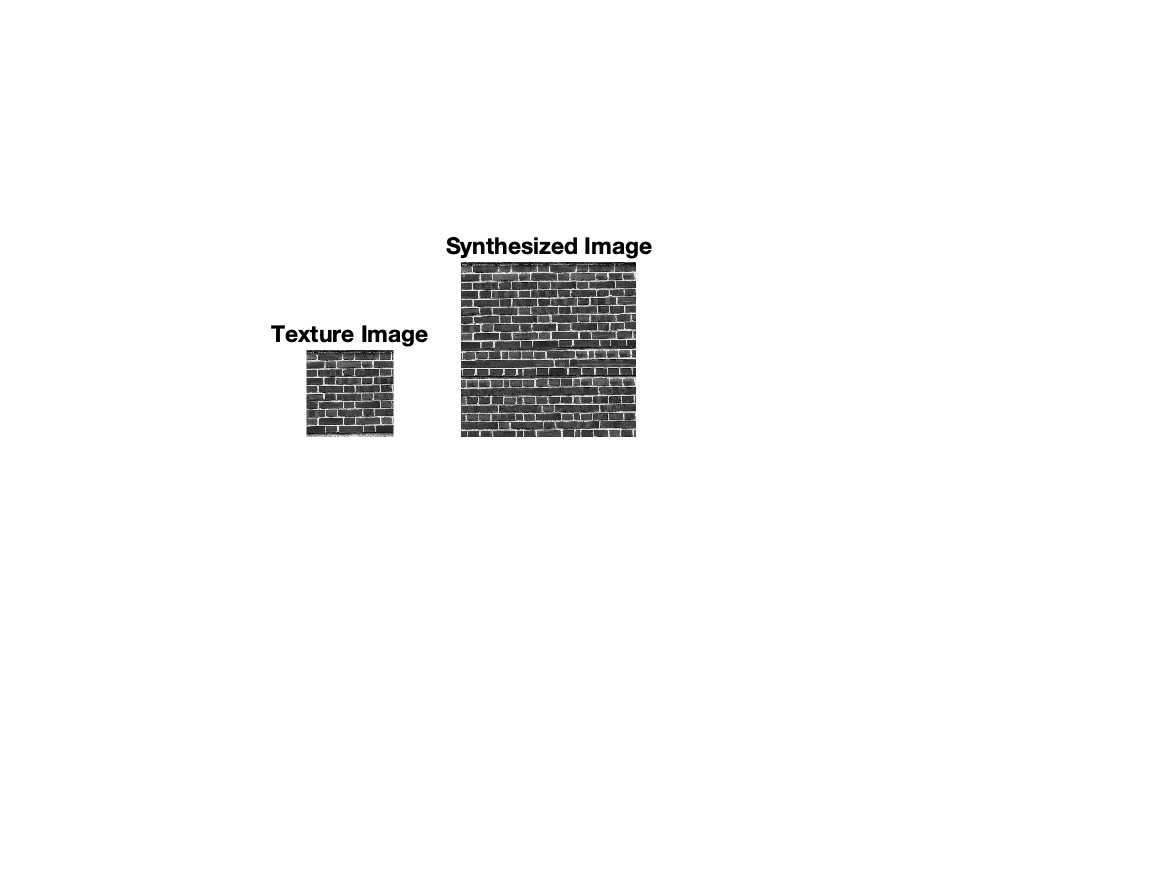
\includegraphics[trim={4.5cm 7cm 8.0cm 3cm}, clip, scale=1.5, width=\textwidth]{../results/syn_final/result_brick_bw_B_40.png}
        \caption{D1}
        \label{fig:d1_res}
    \end{subfigure}
    \hfill
    \begin{subfigure}[h]{0.33\textwidth}
       \centering
       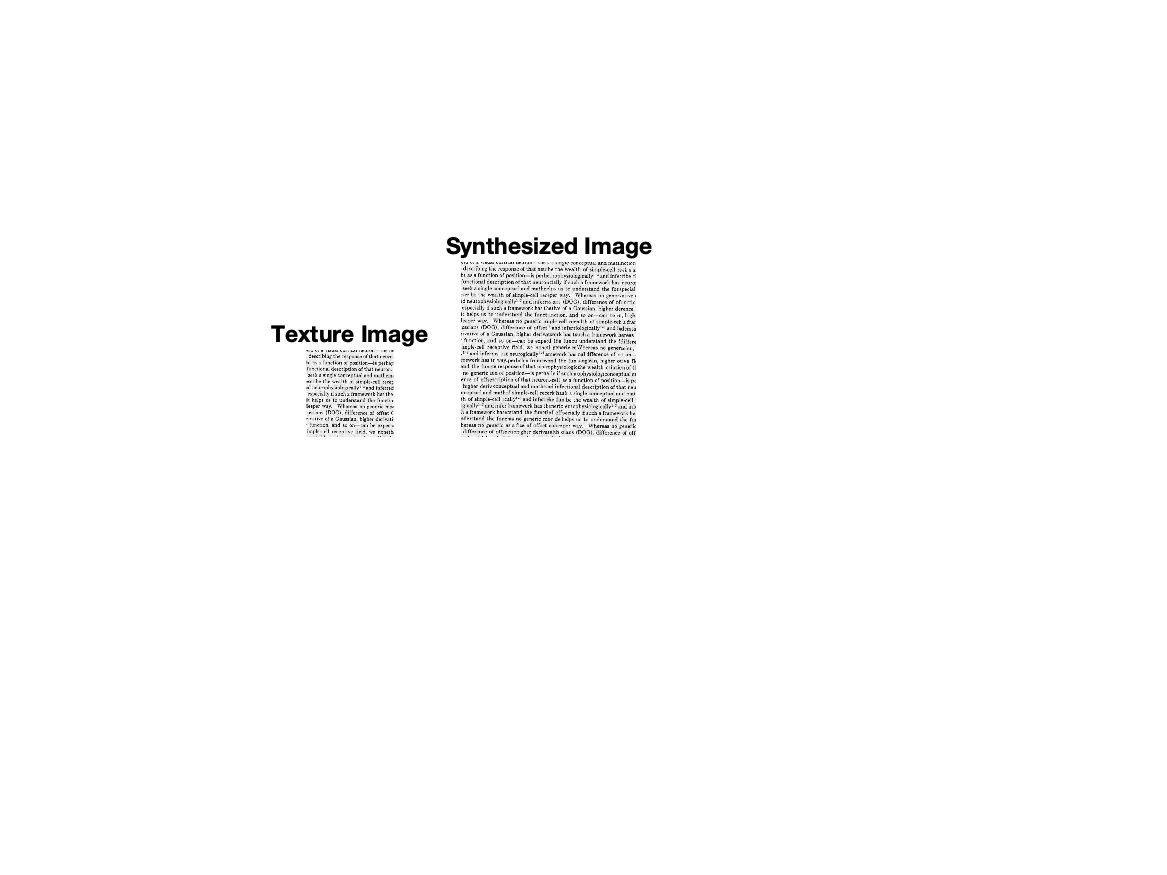
\includegraphics[trim={4.5cm 7cm 8.0cm 3cm}, clip, scale=1.5, width=\textwidth]{../results/syn_final/result_text_B_40.png}
       \caption{text}
       \label{fig:text_res}
   \end{subfigure}
   \hfill
   \begin{subfigure}[h]{0.33\textwidth}
       \centering
       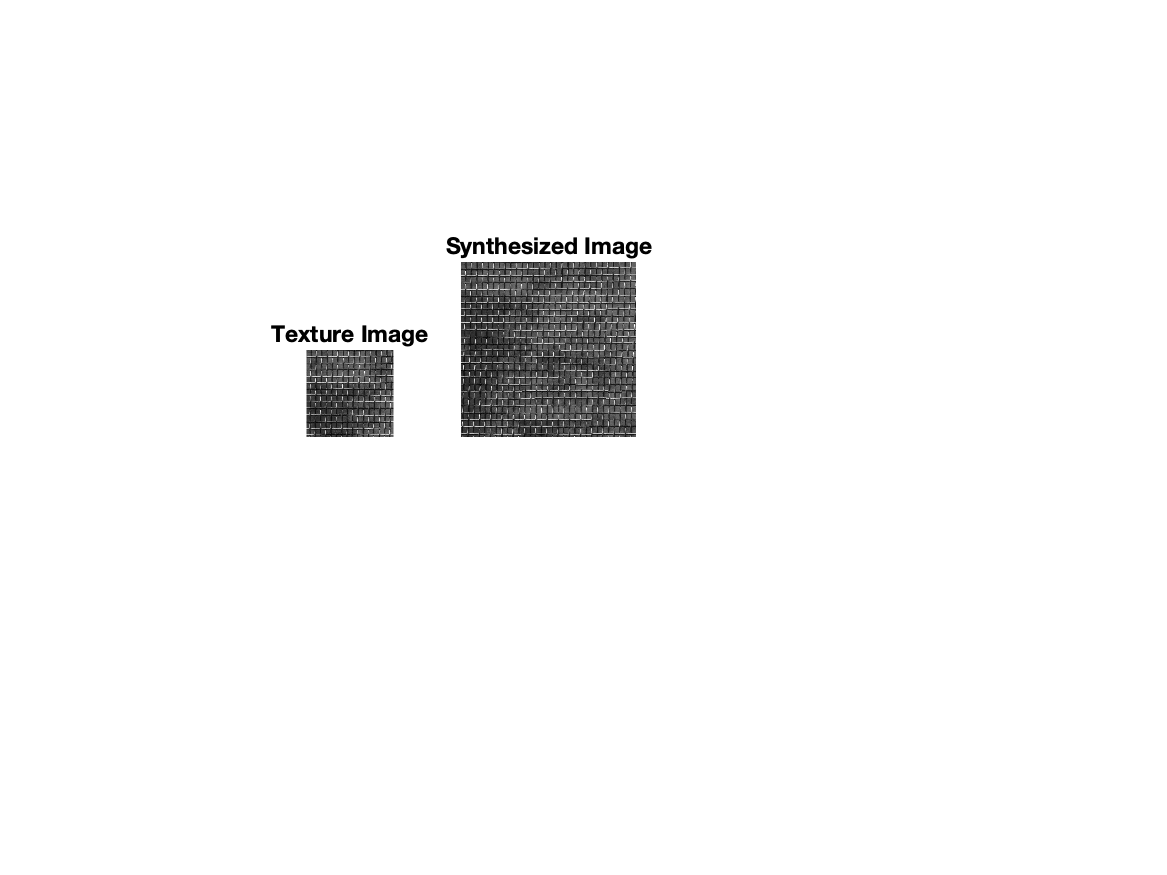
\includegraphics[trim={4.5cm 7cm 8.0cm 3cm}, clip, scale=1.5, width=\textwidth]{../results/syn_final/result_D1_B_40.png}
       \caption{Bricks B/W}
       \label{fig:bricksbw_res}
   \end{subfigure}
   \begin{subfigure}[h]{0.33\textwidth}
         \centering
         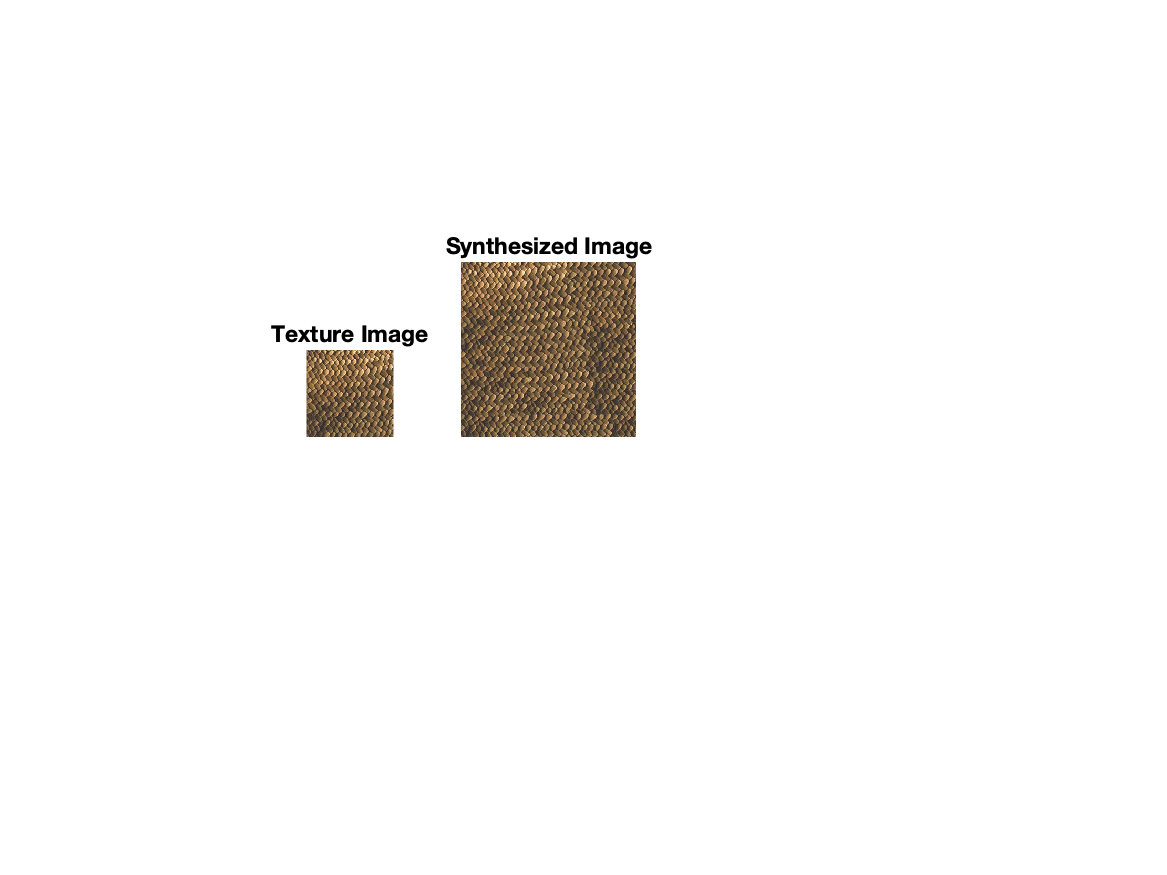
\includegraphics[trim={4.5cm 7cm 8.0cm 3cm}, clip, scale=1.5, width=\textwidth]{../results/syn_final/result_fabric_B_40.png}
         \caption{Fabric}
         \label{fig:apple_res}
     \end{subfigure}
     \hfill
     \begin{subfigure}[h]{0.33\textwidth}
        \centering
        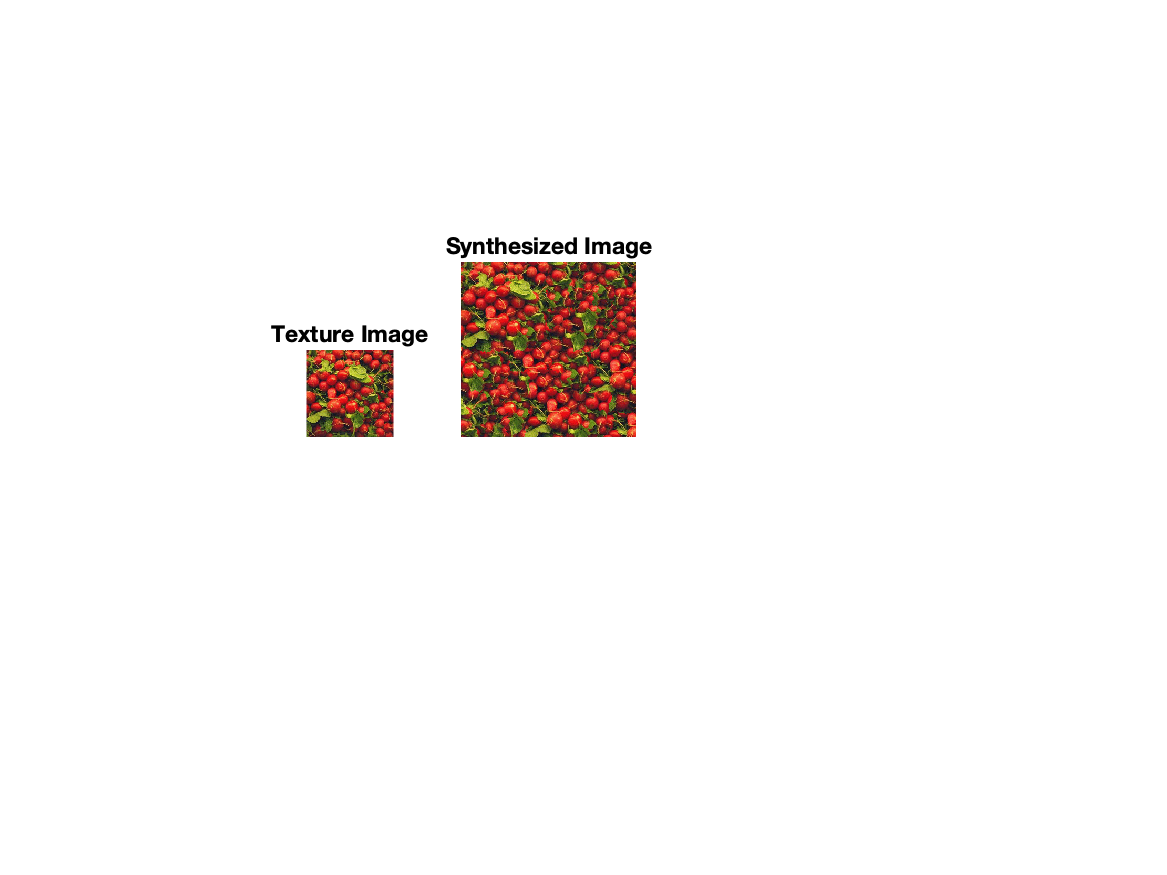
\includegraphics[trim={4.5cm 7cm 8.0cm 3cm}, clip, scale=1.5, width=\textwidth]{../results/syn_final/result_radishes_B_40.png}
        \caption{Radishes}
        \label{fig:apple_res}
    \end{subfigure}
    \hfill
    \begin{subfigure}[h]{0.33\textwidth}
        \centering
        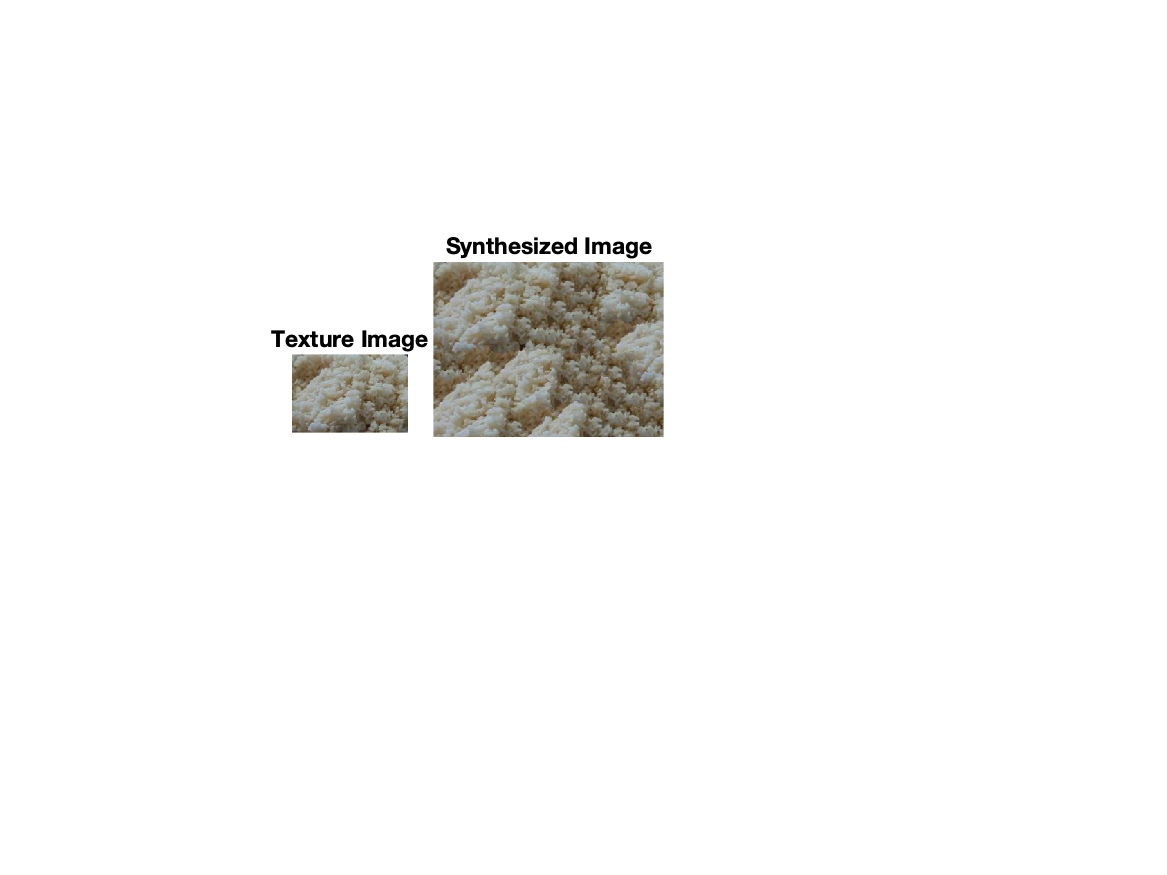
\includegraphics[trim={4.5cm 7cm 8.0cm 3cm}, clip, scale=1.5, width=\textwidth]{../results/syn_final/result_rice_B_40.png}
        \caption{Rice}
        \label{fig:apple_res}
    \end{subfigure}
    \begin{subfigure}[h]{0.33\textwidth}
        \centering
        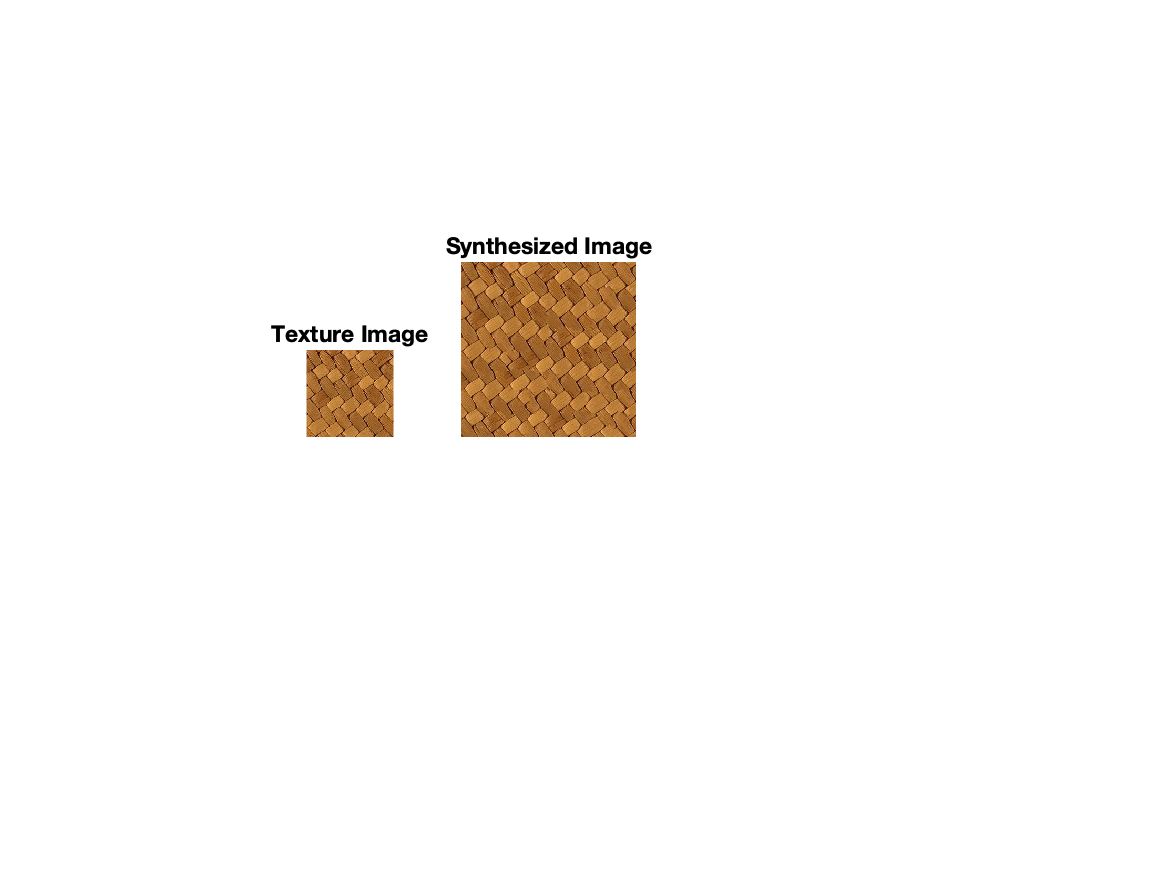
\includegraphics[trim={4.5cm 7cm 8.0cm 3cm}, clip, scale=1.5, width=\textwidth]{../results/syn_final/result_wood_c_B_40.png}
        \caption{Wood}
        \label{fig:apple_res}
    \end{subfigure}
    \hfill
    \begin{subfigure}[h]{0.33\textwidth}
       \centering
       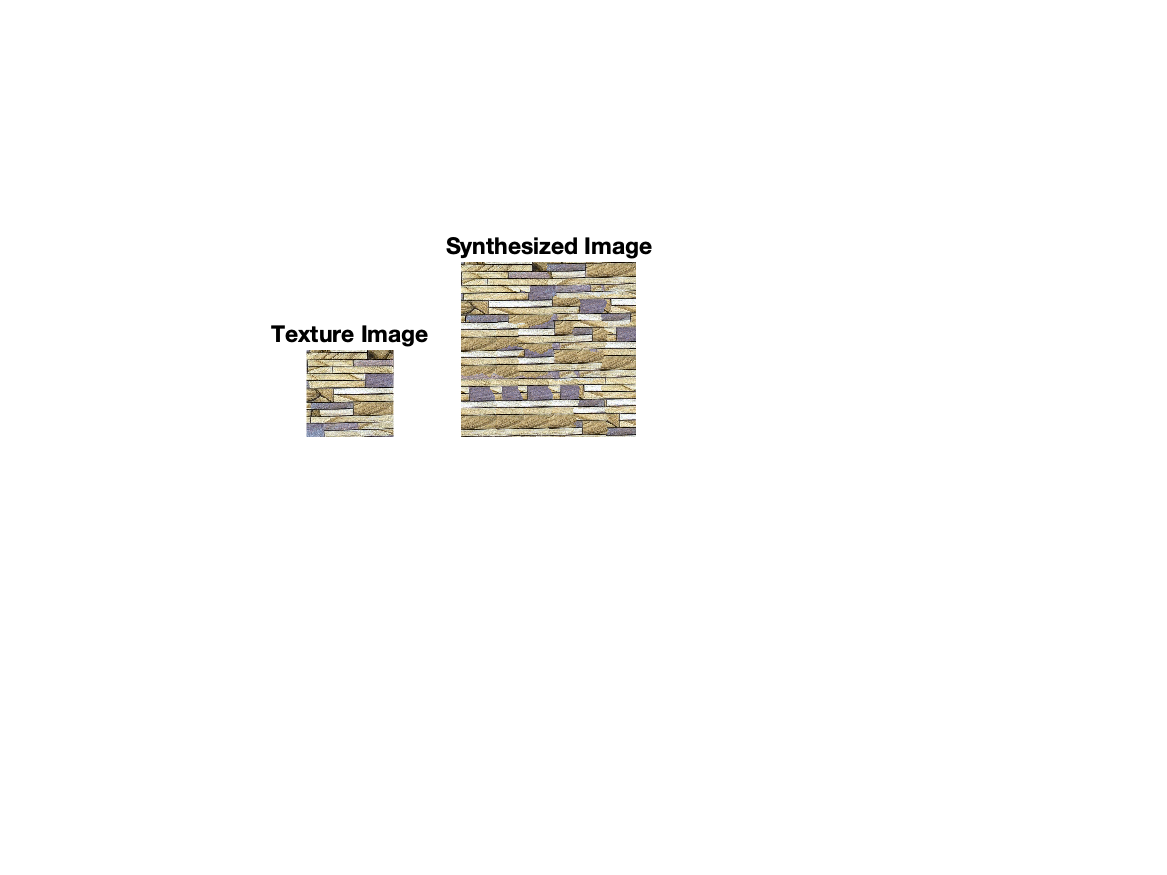
\includegraphics[trim={4.5cm 7cm 8.0cm 3cm}, clip, scale=1.5, width=\textwidth]{../results/syn_final/result_tile_B_60.png}
       \caption{Tiles}
       \label{fig:apple_res}
   \end{subfigure}
   \hfill
   \begin{subfigure}[h]{0.33\textwidth}
       \centering
       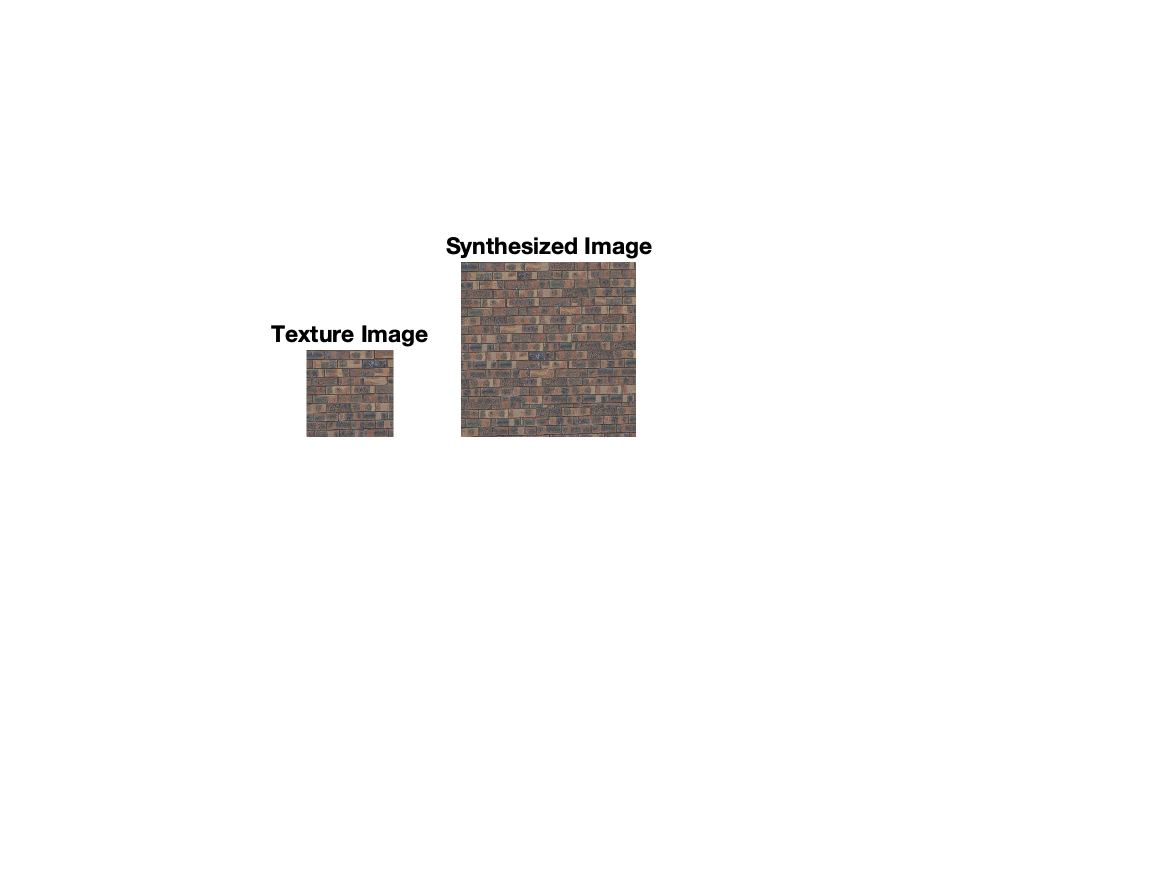
\includegraphics[trim={4.5cm 7cm 8.0cm 3cm}, clip, scale=1.5, width=\textwidth]{../results/syn_final/result_brick_B_60.png}
       \caption{Bricks}
       \label{fig:apple_res}
   \end{subfigure}
   \begin{subfigure}[h]{0.33\textwidth}
    \centering
    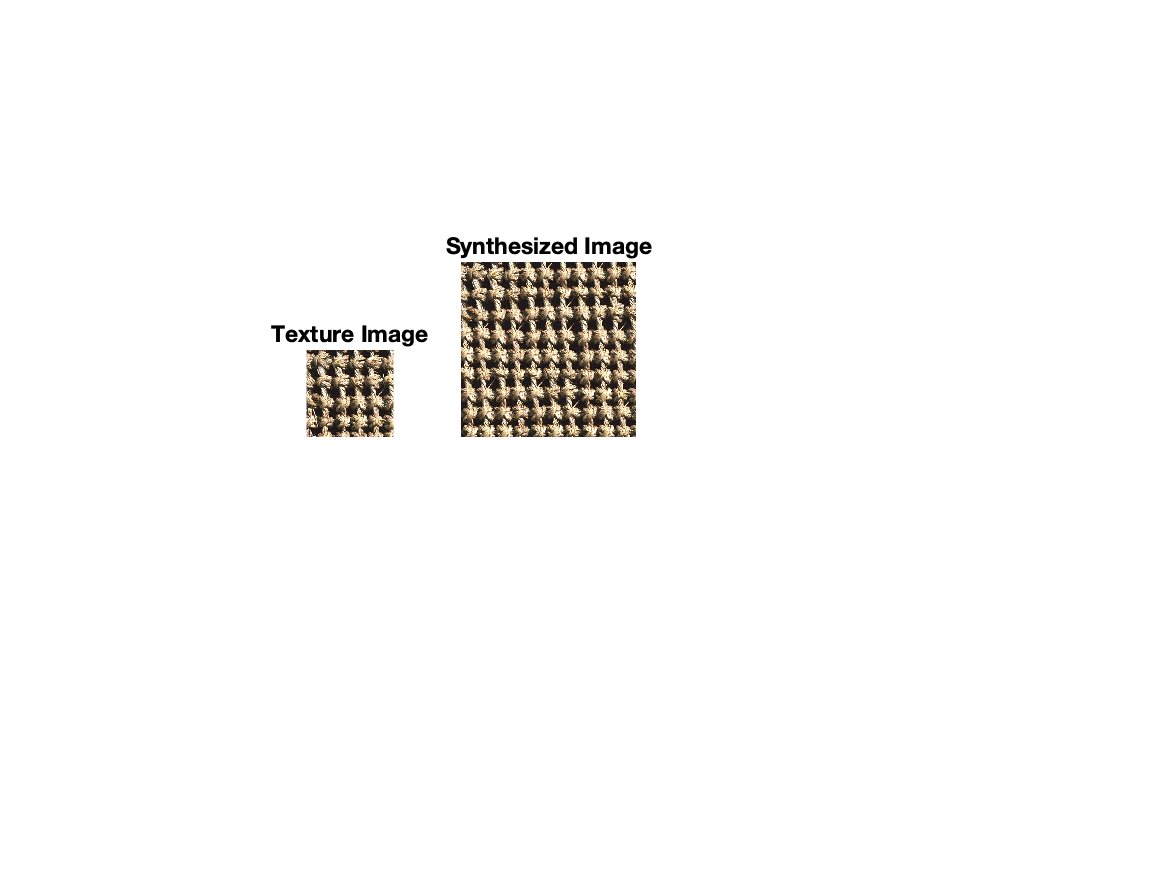
\includegraphics[trim={4.5cm 7cm 8.0cm 3cm}, clip, scale=1.5, width=\textwidth]{../results/syn_final/result_rope_B_60.png}
    \caption{Rope}
    \label{fig:apple_res}
\end{subfigure}
\hfill
\begin{subfigure}[h]{0.33\textwidth}
   \centering
   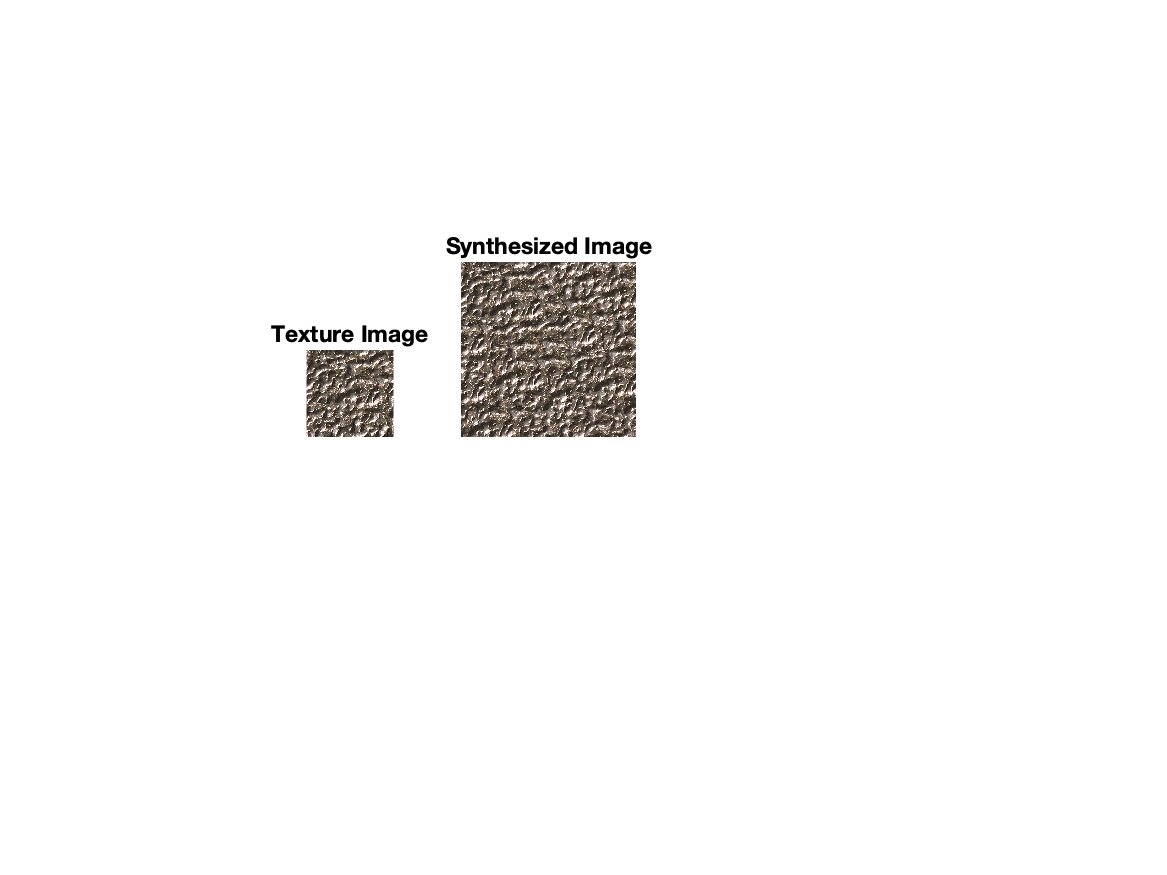
\includegraphics[trim={4.5cm 7cm 8.0cm 3cm}, clip, scale=1.5, width=\textwidth]{../results/syn_final/result_br_pattern_B_60.png}
   \caption{Pattern}
   \label{fig:apple_res}
\end{subfigure}
\hfill
\begin{subfigure}[h]{0.33\textwidth}
   \centering
   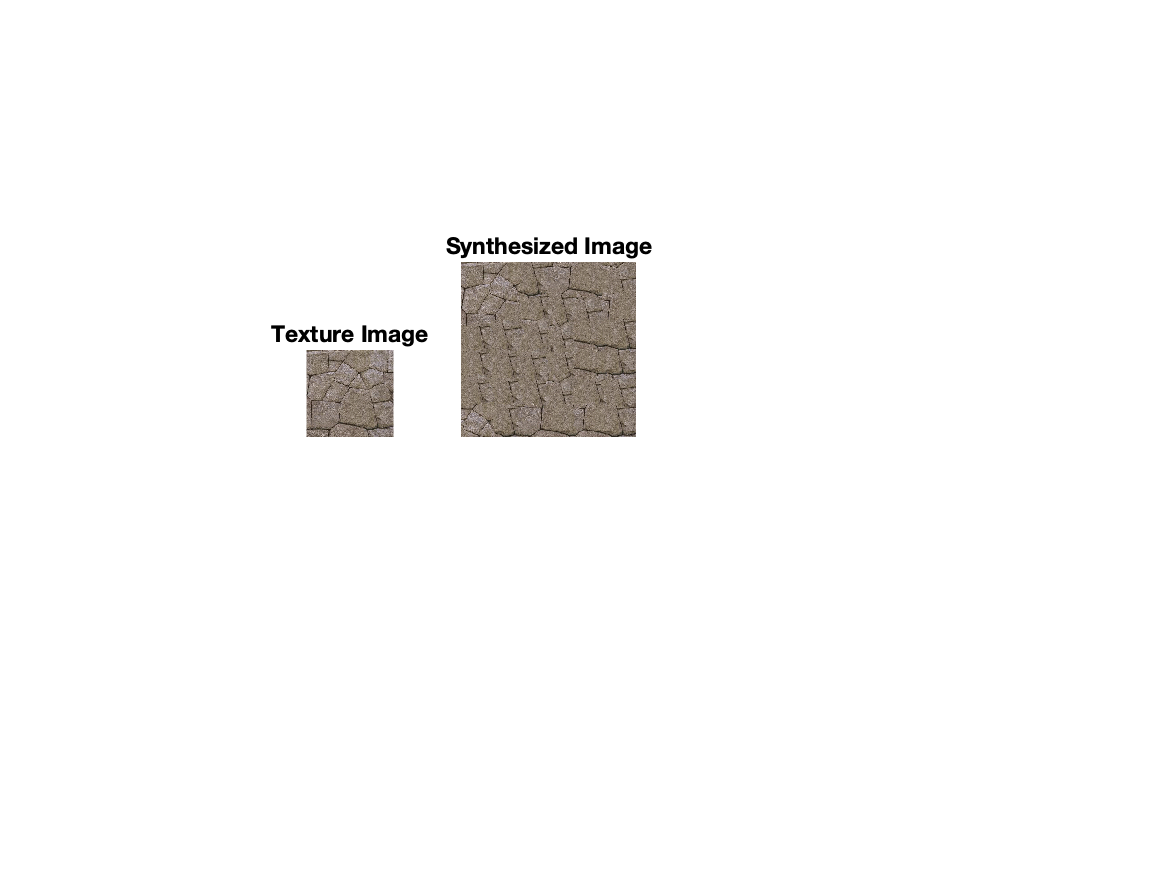
\includegraphics[trim={4.5cm 7cm 8.0cm 3cm}, clip, scale=1.5, width=\textwidth]{../results/syn_final/result_stone_B_60.png}
   \caption{Stone}
   \label{fig:apple_res}
\end{subfigure}   
       \caption{Quilting Results}
        \label{fig:quil_final}
\end{figure*}


% \begin{thebibliography}{999}

% \bibitem{one}
% https://www.geeksforgeeks.org/deep-q-learning/

% \bibitem{two}
% https://www.cs.swarthmore.edu/~bryce/cs63/s16/slides/3-25approximateQ-learning.pdf
% main ref for QL: 
% \bibitem{three}
% http://www.gatsby.ucl.ac.uk/~dayan/papers/cjch.pdf
% \bibitem{four}
% https://courses.cs.washington.edu/courses/cse473/16au/slides-16au/18-approx-rl2.pdf
% \bibitem{five}
% https://www.intel.ai/demystifying-deep-reinforcement-learning/\#gs.hxyudi
% \bibitem{six}
% https://pdfs.semanticscholar.org/2d7e/7d809af7d68c.pdf
% \bibitem{seven}
% https://github.com/moduIo/Deep-Q-network
% \bibitem{eight}
% https://towardsdatascience.com/advanced-dqns-playing-pac-man-with-deep-reinforcement-learning-3ffbd99e0814
% \bibitem{nine}
% {https://lilianweng.github.io/lil-log/2018/05/05/implementing-deep-reinforcement-learning-models.html}
% \bibitem{ten}{https://gym.openai.com/envs/MsPacman-v0/}
% \bibitem{eleven}{https://github.com/gauravmittal1995/Pyman}
% \bibitem{twelve}{https://pythonprogramming.net/pygame-python-3-part-1-intro/}
% \bibitem{thirteen}{https://oregonstate.instructure.com }
% \end{thebibliography}
\end{document}
